\documentclass{beamer}
\setbeamertemplate{navigation symbols}{}

\usepackage{beamerthemeshadow}
\usepackage{amsmath}
\usepackage{bm}

\begin{document}
\title{Information bounds and attractor dynamics of a Hebbian associative memory}  
\author{Clayton Seitz}
\date{\today} 

\begin{frame}[plain]
\titlepage
\end{frame}

\begin{frame}[plain]
\frametitle{RNNs trained with a Hebbian learning rule}

\begin{center}
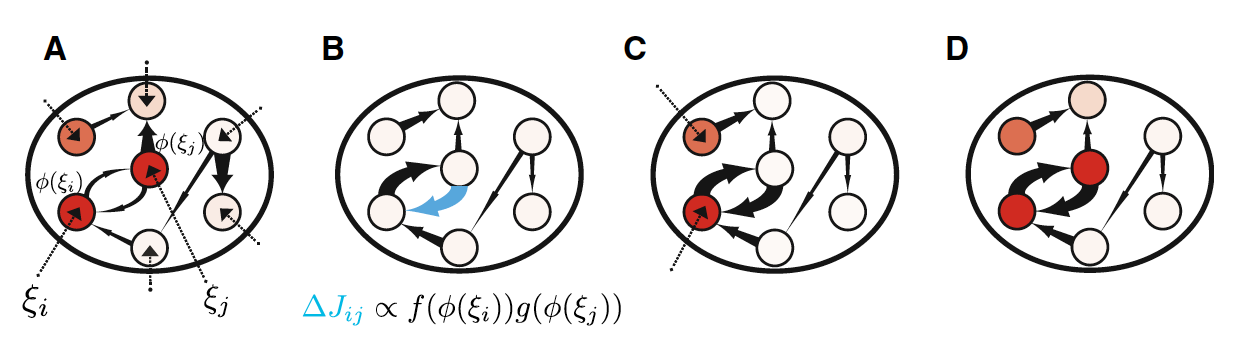
\includegraphics[scale=0.5]{network-diagram}
\end{center}

Measure $\Delta r$ to infer the learning rule $\Delta W_{ij}$. 

\footnote{\cite{peirera}}

\end{frame}


\begin{frame}[plain]
\frametitle{Inferring the transfer function from ITC data}

\vspace{0.2in}

\begin{center}
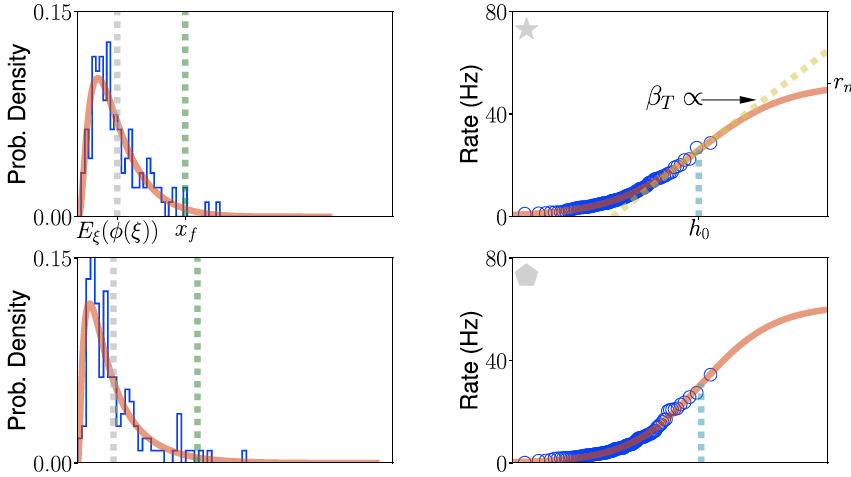
\includegraphics[scale=0.5]{transfer-function}
\end{center}

Measuring the \emph{static} transfer function from novel images assuming that input currents are Gaussian variables

\begin{equation*}
\phi(\bm{\xi}) = \frac{r_{max}}{1 + \exp \beta (\bm{\xi}- \bm{\xi}_{0})}
\end{equation*}


\footnote{\cite{peirera}}
\end{frame}

\begin{frame}[plain]
\frametitle{Inferring the learning rule from ITC data}

\begin{center}
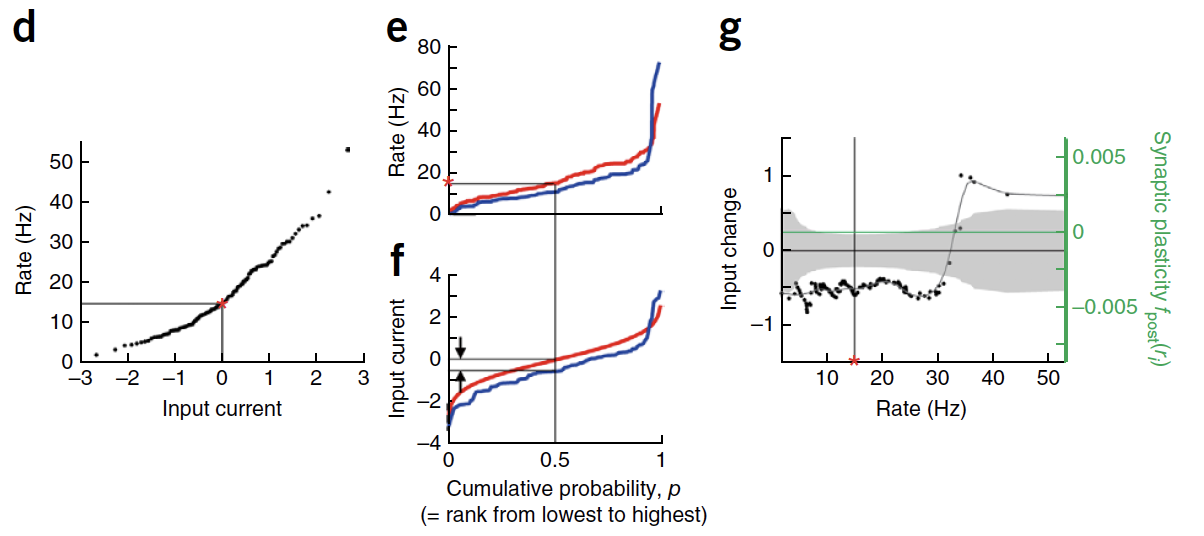
\includegraphics[scale=0.55]{learning-rules}
\end{center}

Inferring the change in input current $\xi_{in}$ from the change in firing rate in {\color{red} novel} relative to {\color{blue} familiar} stimuli

\footnote{\cite{lim}}

\end{frame}

\begin{frame}[plain]
\frametitle{Inferring the learning rule from ITC data}

\begin{center}
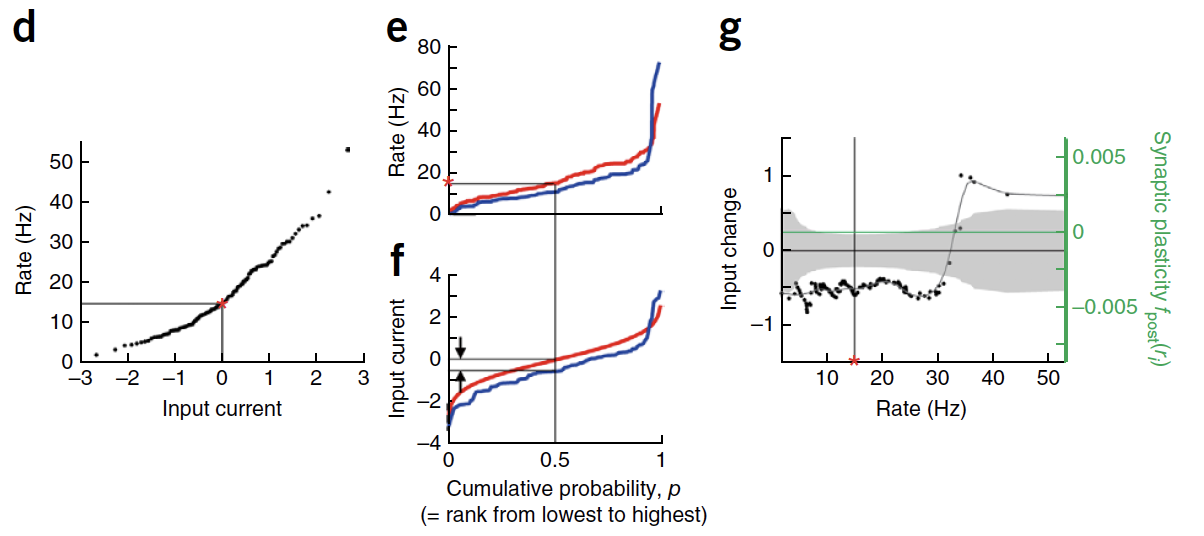
\includegraphics[scale=0.55]{learning-rules}
\end{center}

The change in input current to a neuron can then be read from the firing rate of that neuron when presented a novel stimulus

\begin{align*}
\Delta \xi_{i}(r) \propto (2q + 1 - \tanh (\beta (r-x)))
\end{align*}

\footnote{\cite{lim}}

\end{frame}

\begin{frame}[plain]
\frametitle{A Hebbian update for synaptic weights}

Assuming that $\Delta W_{ij} \propto f(r_{i})g(r_{j})$, the change in input current is related to synaptic plasticity by

\begin{equation*}
\Delta \xi_{i}  \propto  f(r_{i}) \sum_{j} g(r_{j})r_{j}
\end{equation*}

which we have fit from the data as 

\begin{align*}
\Delta \xi_{i}(r) \propto (2q + 1 - \tanh (\beta (r-x)))
\end{align*}

so we can write

\begin{align*}
f(r_{i}) =  \frac{(2q + 1 - \tanh (\beta (r-x)))}{\sum_{j} g(r_{j})r_{j}}\\
\end{align*}


\end{frame}

\begin{frame}[plain]
\frametitle{A Hebbian update for synaptic weights}

During training, we stimulate the network with

\begin{equation*}
\xi_{in}(\bm{\mu}, \bm{\Sigma}) = \frac{1}{(2\pi)^{n/2}|\bm{\Sigma}|^{1/2}}\exp-\frac{1}{2}(\bm{r}-\bm{\mu})^{T}\bm{\Sigma}^{-1}(\bm{r}-\bm{\mu})
\end{equation*}



\footnote{\cite{hopfield}}
\end{frame}


\begin{frame}[plain]
\frametitle{Presenting novel and familiar stimuli to the network}

\vspace{0.2in}

\begin{center}
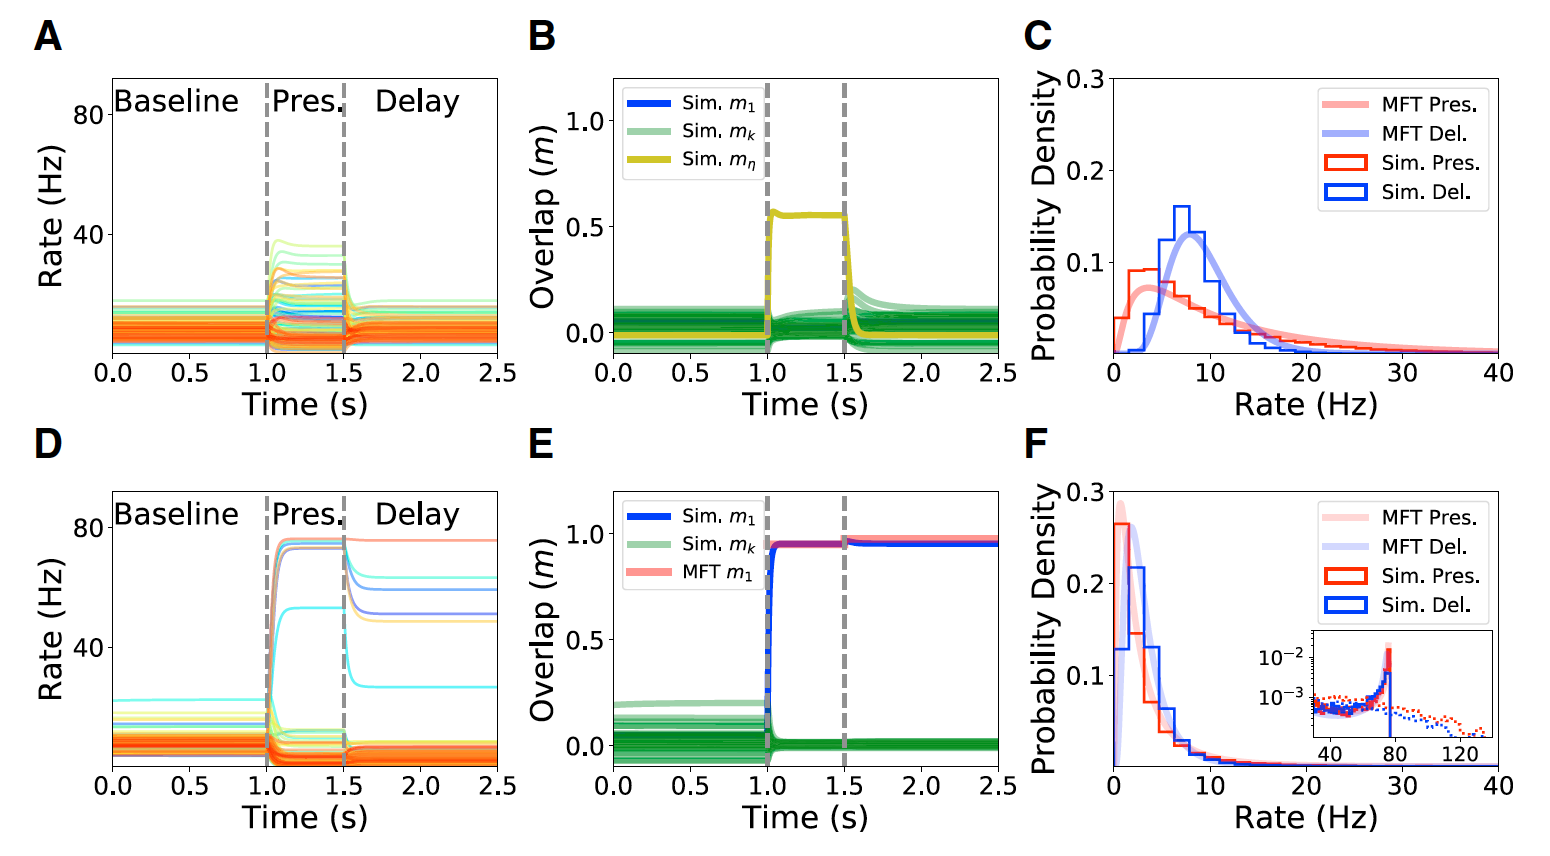
\includegraphics[scale=0.4]{novel-familiar}
\end{center}

\footnote{\cite{peirera}}

\end{frame}

\begin{frame}[plain]
\frametitle{Do these networks optimize information transmission?} 

Are these networks functioning at a critical point? What about the balance between input and recurrence? (Cramer et al. 2020)

\begin{center}
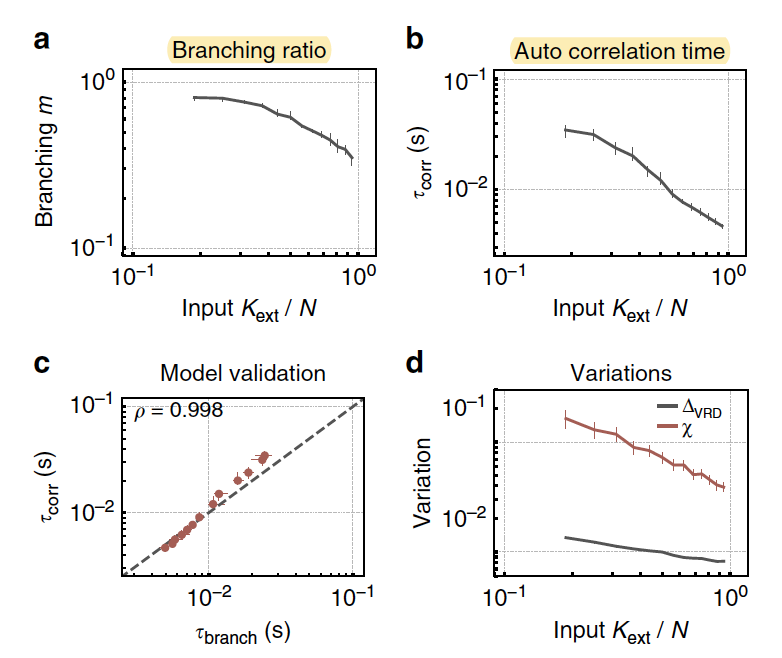
\includegraphics[scale=0.55]{cramer-criticality}
\end{center}

\end{frame}


\begin{frame}[plain]
\frametitle{A coding theory perspective} 

How much information does the response $R$ carry about the input pattern $S$ i.e. $I(R;S)$ on novel and familiar stimuli?

\vspace{0.2in}

What is the fundamental coding capacity of these networks?

\end{frame}


\begin{thebibliography}{99} 
\bibitem[Peirera and Brunel, Neuron. 2018]{peirera}
\bibitem[Lim et al., Nature Neuroscience. 2015]{lim}
\bibitem[J.J. Hopfield PNAS. 1982]{hopfield}
\end{thebibliography}






\end{document}